\chapter{DEMONSTRATION AND EVALUATION}

\section{Introduction}
\label{sec:ch4-introduction}

This chapter closes the \ac{DSR} lifecycle by putting the artifact built in Chapter~III into operation and measuring it against the three objectives defined in Section~\ref{sec:ch3-objectives}. It is organized in two parts. The first demonstrates the system in action: what it looks like when running, what kinds of questions it can handle, and what its internal pipeline does from the moment a user submits a query to the moment a response is returned. The second part evaluates the results: training outcomes for both models, the quality of the retrieval layer, and compliance with the on-premises deployment constraint.

% ================================================================
% PART I: DEMONSTRATION
% ================================================================
\section{Part I: Demonstration}
\label{sec:ch4-demonstration}

% ----------------------------------------------------------------
\subsection{System Overview at Demo Time}
\label{subsec:ch4-system-overview}

The deployed system is split into two distinct flows that operate at different times. The first is the preparation pipeline described in Part~I of Chapter~III: n8n orchestrates the seven phases (scraping, upload, text extraction, article extraction, validation, embedding, and vector storage) by calling a FastAPI server that triggers each phase on demand. This pipeline runs once per corpus update and has no role at query time; for the purpose of this demonstration, two \ac{JORT} issues from early 2026 have been indexed into Qdrant, constituting a representative proof-of-concept corpus.

\vspace{0.5em}

The second flow is the real-time query pipeline, which handles each user question independently. Table~\ref{tab:system-components} lists the components that are active at query time, with no external network call involved in any of them.

\begin{table}[H]
\centering
\caption{Components Active at Query Time}
\label{tab:system-components}
\renewcommand{\arraystretch}{1.3}
\begin{tabular}{|p{4.5cm}|p{8cm}|}
\hline
\textbf{Component} & \textbf{Role at query time} \\
\hline
BAAI/bge-m3 & Encodes the user query into a dense vector (1,024 dimensions) and a sparse lexical vector simultaneously \\
\hline
Qdrant (\texttt{jort\_articles\_v2}) & Runs a hybrid search over the pre-indexed corpus and returns the top-20 candidate articles \\
\hline
BAAI/bge-reranker-v2-m3 & Scores each (query, article) pair jointly and re-orders the candidates by relevance; score determines whether article context is injected into the prompt \\
\hline
Fine-tuned model via Ollama & Generates the final grounded answer from the selected articles; served locally in \ac{GGUF} q4\_k\_m format \\
\hline
\end{tabular}
\end{table}

Figure~\ref{fig:qdrant-collection} shows the \texttt{jort\_articles\_v2} collection in the Qdrant dashboard after the full corpus has been indexed, confirming that all legal articles are stored and ready for retrieval.

\begin{figure}[H]
\centering
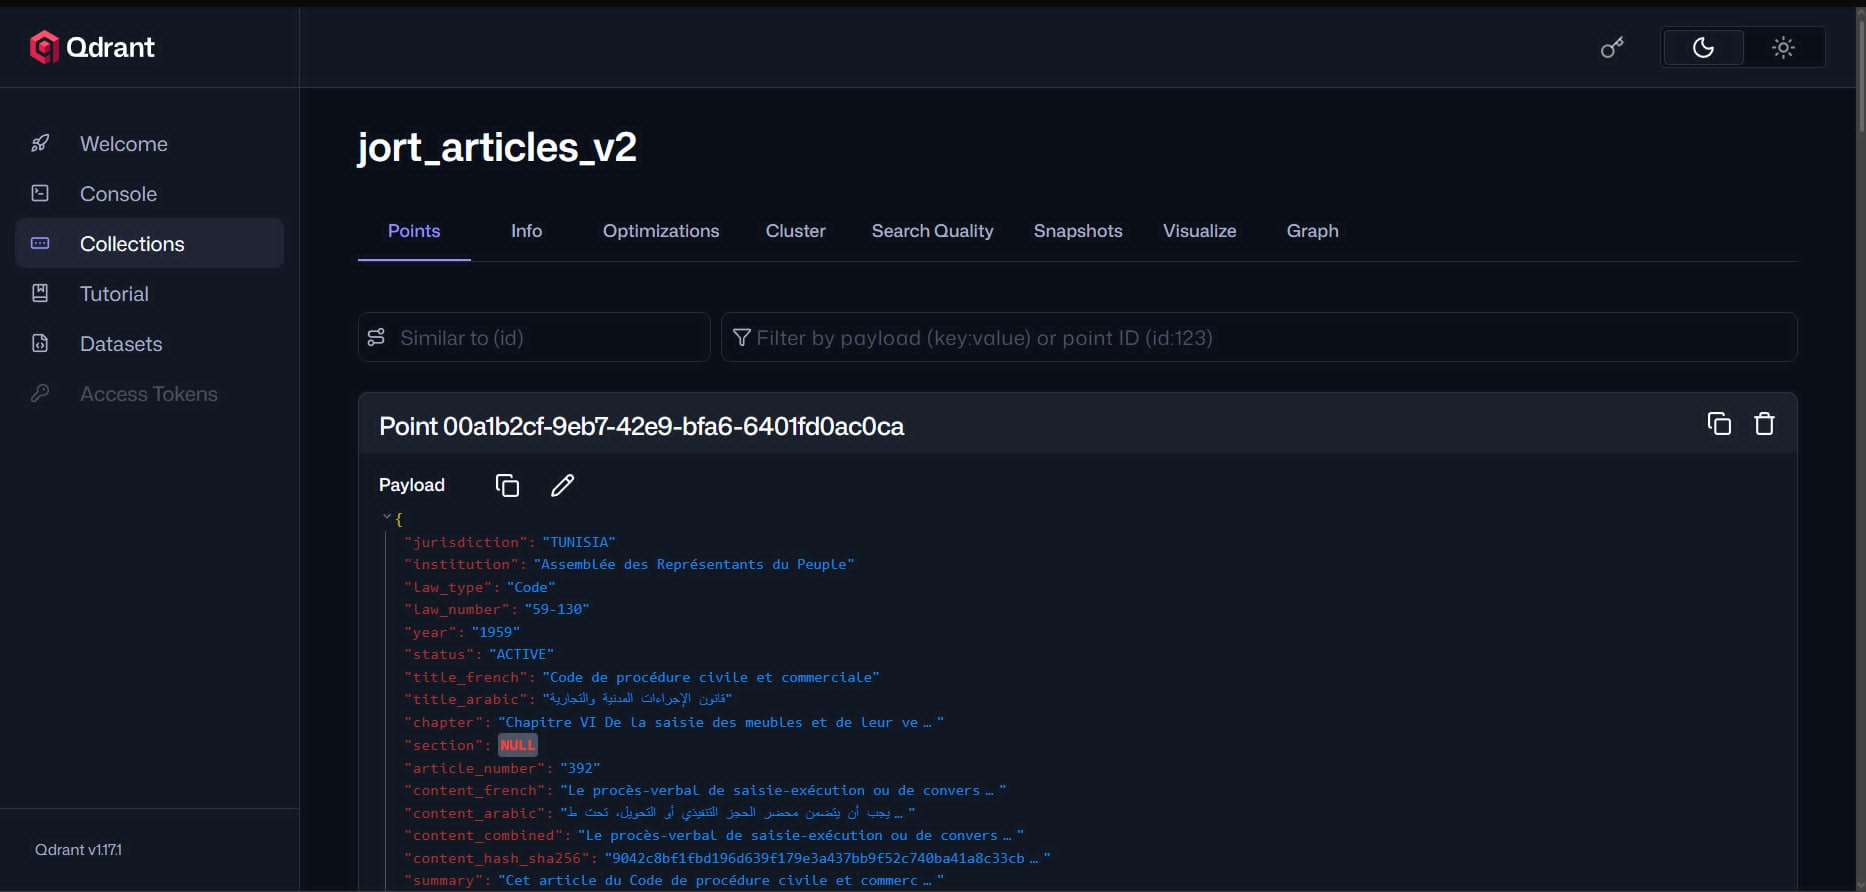
\includegraphics[width=0.85\textwidth]{figures/qdrant_collection.png}
\caption{Qdrant Dashboard Showing the \texttt{jort\_articles\_v2} Collection After Indexing}
\label{fig:qdrant-collection}
\end{figure}

Both fine-tuned models, Gemma~4~E4B and Qwen3.5~9B, are available as \ac{GGUF} files and can be loaded into Ollama interchangeably. The following demonstration was conducted with both models answering the same queries independently.

% ----------------------------------------------------------------
\subsection{Pipeline Execution}
\label{subsec:ch4-n8n-execution}

The preparation pipeline is triggered automatically by a schedule defined in n8n, so new \ac{JORT} issues are picked up and indexed without manual intervention. During development and testing, a manual trigger is used instead to run the pipeline on demand. From the moment the trigger fires, n8n executes each phase in sequence, calling the FastAPI server to start each job and polling its status until it completes before moving to the next phase. To make the pipeline observable without having to watch the n8n UI, a Telegram bot integration sends a notification at the start and end of every phase. These notifications serve as the operational log of each pipeline run.

\vspace{0.5em}

The sequence below shows the notifications received during a representative execution that processed \ac{JORT} issues for the year 2026. Each message was sent automatically by n8n and received in real time on a mobile device.

\vspace{0.5em}

\noindent\textbf{Phase 1 -- Scraping:}

\vspace{0.3em}
\noindent
\begin{minipage}[t]{0.48\textwidth}
\small
\begin{verbatim}
JORT Scraper — job started

Job ID  : a1b2c3d4-e5f6-7890-ab12
Script  : lois_decrets_fr
Years   : 2026 -> 2026
Headless: false
Retries : 2
\end{verbatim}
\end{minipage}
\hfill
\begin{minipage}[t]{0.48\textwidth}
\small
\begin{verbatim}
JORT Scraper — download done

Job ID   : a1b2c3d4-e5f6-7890-ab12
Script   : lois_decrets_fr
Years    : 2026 -> 2026
Finished : 2026-01-15T14:32:07+00:00
\end{verbatim}
\end{minipage}

\vspace{0.8em}
\noindent\textbf{Phase 2 -- Google Drive upload:}

\vspace{0.3em}
\noindent
\begin{minipage}[t]{0.48\textwidth}
\small
\begin{verbatim}
JORT Upload — job started

Job ID : b2c3d4e5-f6a7-8901-bc23
Script : upload_gdrive
\end{verbatim}
\end{minipage}
\hfill
\begin{minipage}[t]{0.48\textwidth}
\small
\begin{verbatim}
JORT Upload — completed

Job ID  : b2c3d4e5-f6a7-8901-bc23
Status  : done
Error   : n/a
Finished: 2026-01-15T14:35:21+00:00
\end{verbatim}
\end{minipage}

\vspace{0.8em}
\noindent\textbf{Phase 3 -- Text extraction:}

\vspace{0.3em}
\noindent
\begin{minipage}[t]{0.48\textwidth}
\small
\begin{verbatim}
JORT Text Extraction — job started

Job ID : c3d4e5f6-a7b8-9012-cd34
Script : text_extraction
\end{verbatim}
\end{minipage}
\hfill
\begin{minipage}[t]{0.48\textwidth}
\small
\begin{verbatim}
JORT Text Extraction — completed

Job ID   : c3d4e5f6-a7b8-9012-cd34
Status   : done
Error    : n/a
Finished : 2026-01-15T14:48:53+00:00
\end{verbatim}
\end{minipage}

\vspace{0.8em}
\noindent\textbf{Phase 4 -- Article extraction:}

\vspace{0.3em}
\noindent
\begin{minipage}[t]{0.48\textwidth}
\small
\begin{verbatim}
JORT Article Extraction — job started

Job ID : d4e5f6a7-b8c9-0123-de45
Script : article_extraction
\end{verbatim}
\end{minipage}
\hfill
\begin{minipage}[t]{0.48\textwidth}
\small
\begin{verbatim}
JORT Article Extraction — completed

Job ID   : d4e5f6a7-b8c9-0123-de45
Status   : done
Error    : n/a
Finished : 2026-01-15T16:12:44+00:00
\end{verbatim}
\end{minipage}

\vspace{0.8em}
\noindent\textbf{Phase 5 -- Validation:}

\vspace{0.3em}
\noindent
\begin{minipage}[t]{0.48\textwidth}
\small
\begin{verbatim}
JORT Validation — job started

Job ID : e4f5a6b7-c8d9-0123-ef45
Script : validation
\end{verbatim}
\end{minipage}
\hfill
\begin{minipage}[t]{0.48\textwidth}
\small
\begin{verbatim}
JORT Validation — completed

Job ID   : e4f5a6b7-c8d9-0123-ef45
Status   : done
Error    : n/a
Finished : 2026-01-15T16:31:08+00:00
\end{verbatim}
\end{minipage}

\vspace{0.8em}
\noindent\textbf{Phase 6 -- Embedding:}

\vspace{0.3em}
\noindent
\begin{minipage}[t]{0.48\textwidth}
\small
\begin{verbatim}
JORT Embedding — job started

Job ID : e5f6a7b8-c9d0-1234-ef56
Script : embedding
Model  : BAAI/bge-m3
\end{verbatim}
\end{minipage}
\hfill
\begin{minipage}[t]{0.48\textwidth}
\small
\begin{verbatim}
JORT Embedding — completed

Job ID   : e5f6a7b8-c9d0-1234-ef56
Status   : done
Error    : n/a
Finished : 2026-01-15T17:01:19+00:00
\end{verbatim}
\end{minipage}

\vspace{0.8em}
\noindent\textbf{Phase 7 -- Vector storage:}

\vspace{0.3em}
\noindent
\begin{minipage}[t]{0.48\textwidth}
\small
\begin{verbatim}
JORT Vector Storage — job started

Job ID     : f6a7b8c9-d0e1-2345-fg67
Script     : vector_storage
Collection : jort_articles_v2
\end{verbatim}
\end{minipage}
\hfill
\begin{minipage}[t]{0.48\textwidth}
\small
\begin{verbatim}
JORT Vector Storage — completed

Job ID   : f6a7b8c9-d0e1-2345-fg67
Status   : done
Error    : n/a
Finished : 2026-01-15T17:08:33+00:00
\end{verbatim}
\end{minipage}

\vspace{0.5em}

Figure~\ref{fig:telegram-notifications} shows the Telegram bot as it appeared during an actual pipeline run, with the sequence of phase notifications received in real time.

\begin{figure}[H]
\centering
\begin{minipage}[t]{0.47\textwidth}
  \centering
  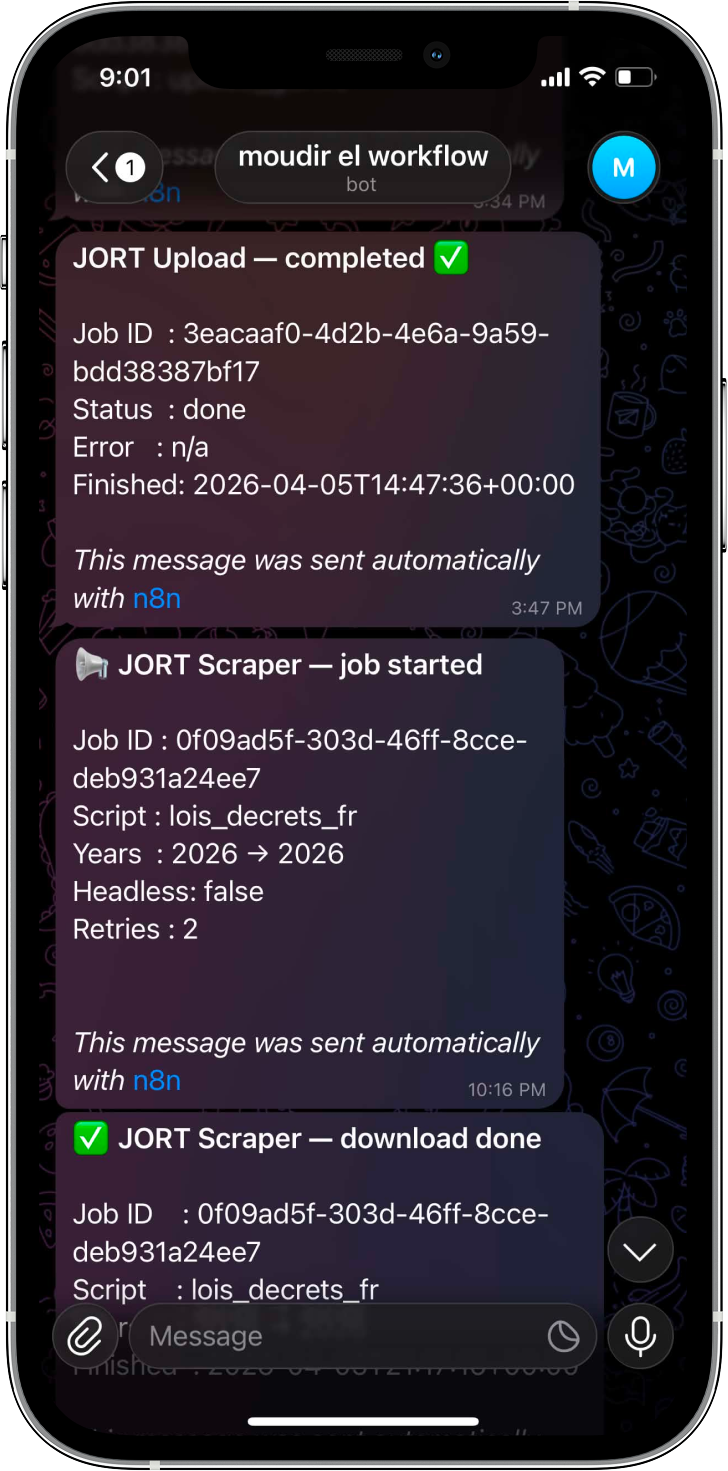
\includegraphics[width=\linewidth]{figures/telegram_1.png}
\end{minipage}
\hfill
\begin{minipage}[t]{0.47\textwidth}
  \centering
  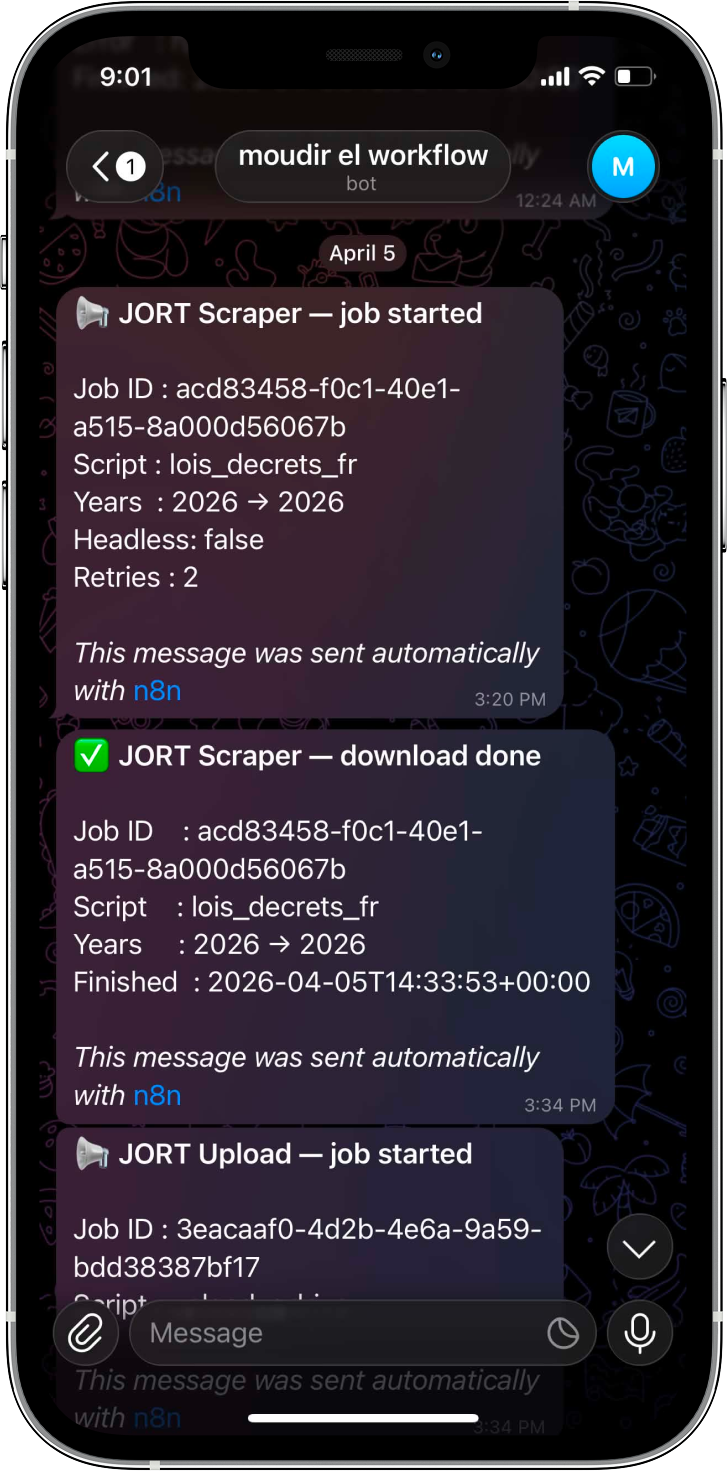
\includegraphics[width=\linewidth]{figures/telegram_2.png}
\end{minipage}
\caption{Telegram Notifications Received During Pipeline Execution}
\label{fig:telegram-notifications}
\end{figure}

Each notification is delivered as soon as the FastAPI job status transitions to \texttt{done}. If a phase fails, the notification reports the error message returned by the FastAPI server, and n8n halts the workflow rather than proceeding to the next phase. This gives immediate visibility into any failure without needing to inspect server logs directly.

\vspace{0.5em}

Figure~\ref{fig:n8n-logs} shows the n8n execution panel during the same pipeline run, with each node marked as successfully executed. Figure~\ref{fig:fastapi-logs} shows the FastAPI server terminal output, confirming that each job was received, queued, and completed without error.

\begin{figure}[H]
\centering
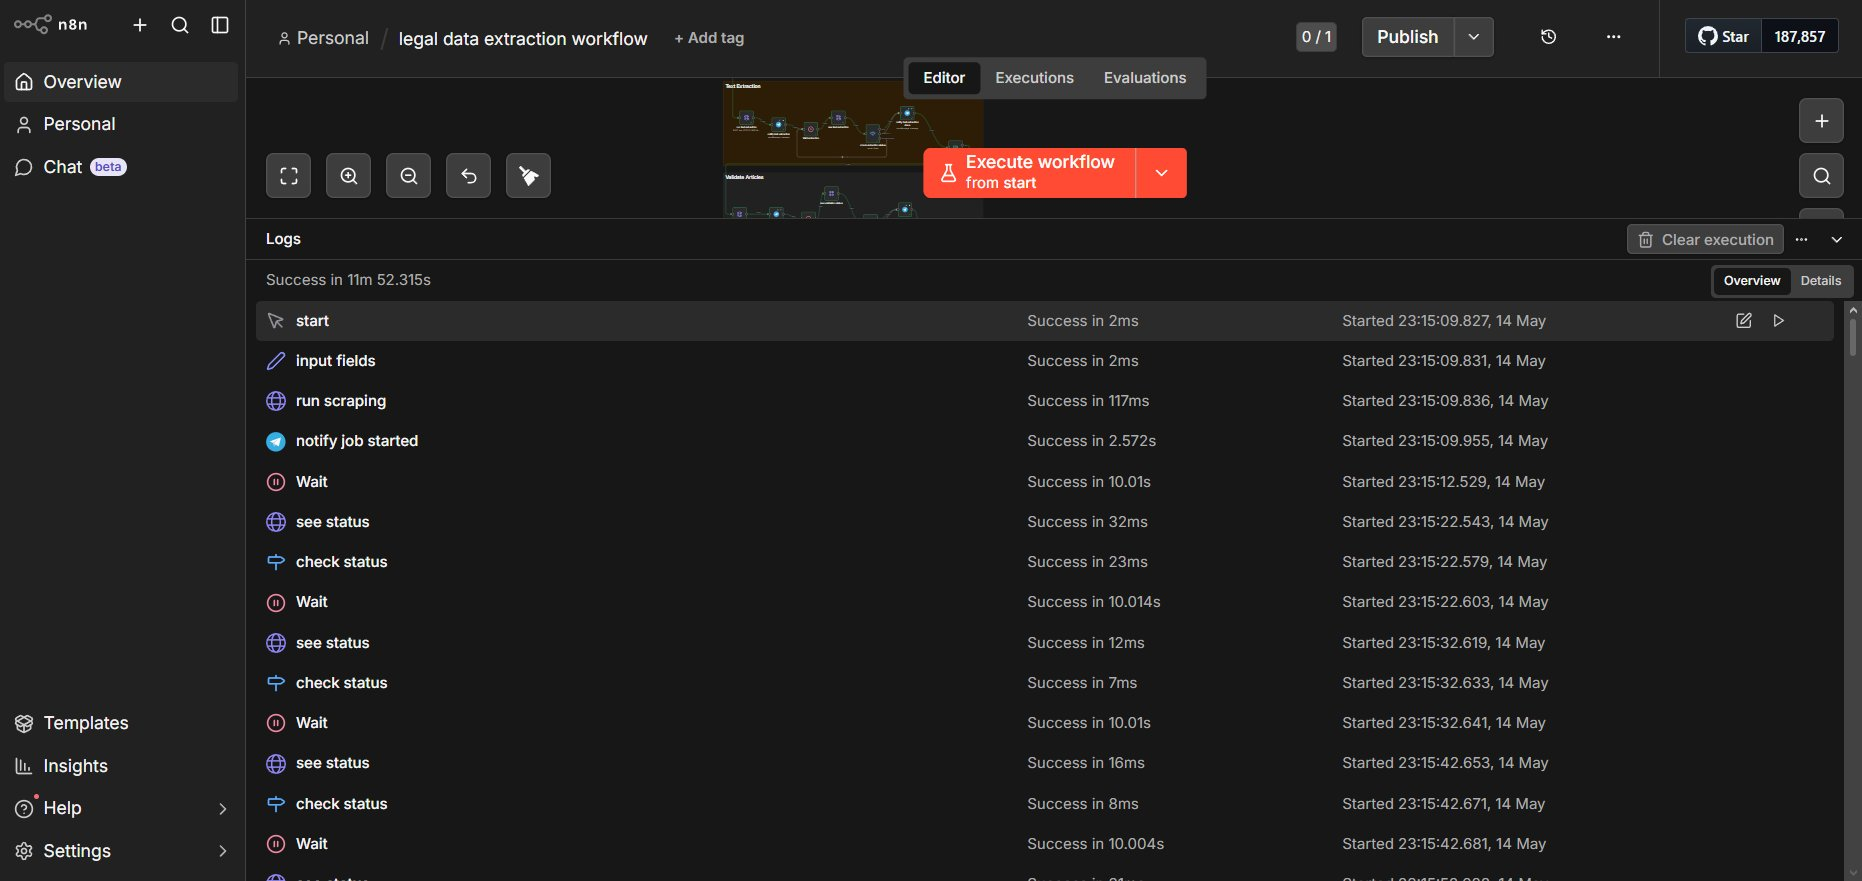
\includegraphics[width=1\textwidth]{figures/n8n_logs.png}
\caption{n8n Execution Panel During Pipeline Run}
\label{fig:n8n-logs}
\end{figure}

\begin{figure}[H]
\centering
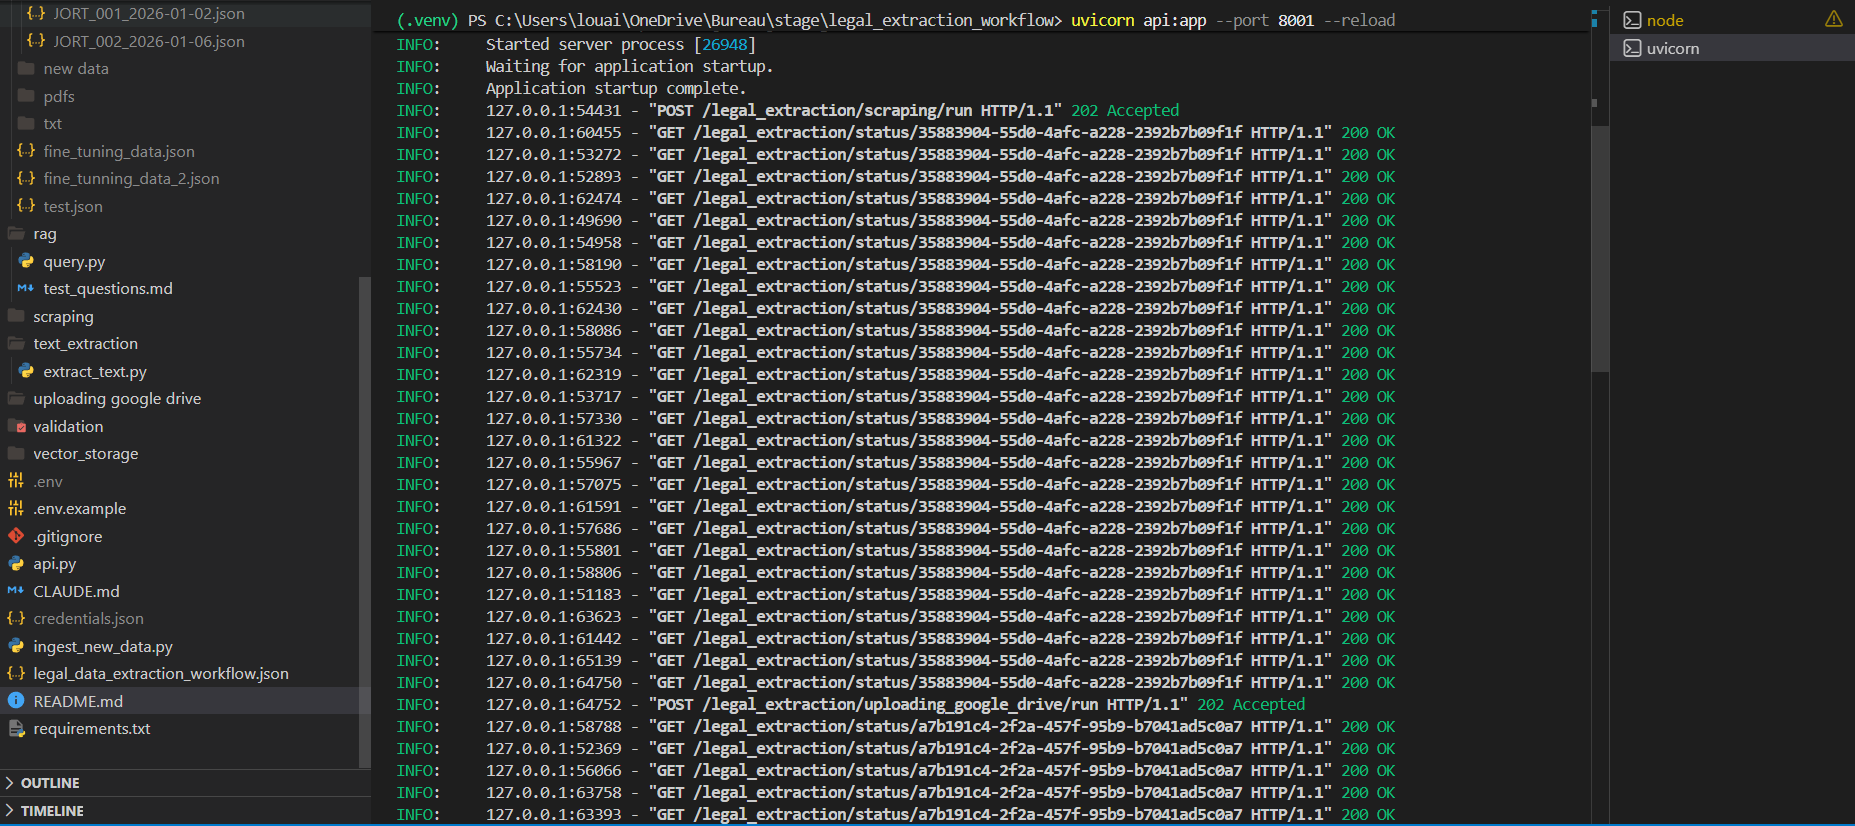
\includegraphics[width=1\textwidth]{figures/fastAPI_logs.png}
\caption{FastAPI Server Logs During Pipeline Run}
\label{fig:fastapi-logs}
\end{figure}

% ----------------------------------------------------------------
\subsection{Example Queries and System Responses}
\label{subsec:ch4-example-queries}

The examples below cover four query categories. The first is drawn from the post-training verification test run at the end of each training run and demonstrates citation and disclaimer conventions. The remaining three target the indexed \ac{JORT} corpus directly and demonstrate retrieval accuracy, multilingual support, and out-of-scope handling.

\subsubsection{Query 1: Contract Validity Under Tunisian Law (French, Direct QA)}
\label{subsubsec:ch4-query1}

This query targets Article~2 of the Code des Obligations et des Contrats (COC), one of the foundational articles of Tunisian contract law, and was used as the standard test case at the end of both training runs.

\vspace{0.5em}

\noindent\textbf{User question:}

\begin{quote}
\textit{Quelles sont les conditions pour qu'un contrat soit valable en droit tunisien?}
\end{quote}

\noindent\textbf{Relevant document passed to the model:}

\begin{quote}
\textit{Article 2 du Code des obligations et des contrats (COC)}
\end{quote}

\vspace{0.5em}

\noindent\textbf{Gemma~4~E4B response:}

\begin{quote}
En vertu de l'article~2 du Code des obligations et des contrats, quatre conditions sont
nécessaires à la validité d'un contrat né d'une déclaration de volonté~: la capacité des
parties à s'obliger, une déclaration de volonté valable portant sur les éléments essentiels
du contrat, un objet certain pouvant former objet d'obligation, et une cause licite.
Par ailleurs, ces conditions doivent être réunies pour que le contrat produise ses effets
juridiques entre les parties. Ainsi, l'absence de l'une de ces conditions peut entraîner
la nullité ou l'inopposabilité du contrat.
Sources~: art.~2 du COC. Ceci ne constitue pas un avis juridique. Pour votre situation
spécifique, consultez un avocat.

\end{quote}

\noindent\textbf{Qwen3.5~9B response:}

\begin{quote}
En vertu de l'article 2 du Code des obligations et des contrats, la validité d'une obligation contractuelle repose sur quatre conditions cumulatives : la capacité de s'obliger, une déclaration de volonté valable portant sur les éléments essentiels, un objet certain, et une cause licite. Ces éléments constituent le socle de la validité contractuelle en droit tunisien. Sources: art. 2 du COC. Ceci ne constitue pas un avis juridique. Pour votre situation spécifique, consultez un avocat
\end{quote}

Both models correctly identified all four conditions stated in Article~2 of the COC, cited the correct source, and appended the mandatory legal disclaimer. The phrasing differs slightly between the two responses: Gemma's answer is structured around the notion of a ``contract born of a declaration of will,'' while Qwen's frames it as conditions for the validity of a ``contractual obligation.'' Both formulations are legally accurate and reflect the article's content faithfully, demonstrating that the fine-tuning has transferred the expected citation and disclaimer conventions to both models.

% ----------------------------------------------------------------
\subsubsection{Query 2: Diploma Conditions for an Archives Examination (French, JORT Corpus)}
\label{subsubsec:ch4-query2}

This query targets the indexed \ac{JORT} corpus directly and verifies that the retrieval pipeline surfaces the correct article for a factual question about a public-sector recruitment examination.

\vspace{0.5em}

\noindent\textbf{User question:}

\begin{quote}
\textit{Quelles sont les conditions de diplôme pour participer au concours de gestionnaire de documents et d'archives ?}
\end{quote}

\noindent\textbf{Relevant document retrieved:}

\begin{quote}
\textit{Article premier de l'arrêté du Conseil national des régions et des districts, JORT n\textsuperscript{o}~2 du 6 janvier 2026}
\end{quote}

\vspace{0.5em}

\noindent\textbf{Gemma~4~E4B response:}

\begin{quote}
En vertu de l'article~1 du décret du 5~janvier~2026, le concours externe de gestionnaire de documents et d'archives est ouvert aux candidats titulaires d'un diplôme de spécialité. Deux parcours sont possibles~: soit un cycle d'études supérieures d'au moins deux~(2) ans aboutissant à un diplôme en gestion des documents et des archives~; soit un cycle de quatre~(4) ans aboutissant à une maîtrise en bibliothéconomie, documentation et archivistique. Une dispense est accordée si le diplôme de formation est homologué au niveau requis. Par ailleurs, les candidats doivent être âgés de 40~ans au plus.
Sources~: art.~1 du décret n\textsuperscript{o}~2026-2000 du 5~janvier~2026. Ceci ne constitue pas un avis juridique. Pour votre situation spécifique, consultez un avocat.
\end{quote}

\noindent\textbf{Qwen3.5~9B response:}

\begin{quote}
Conformément à l'article premier de l'arrêté du Conseil national des régions et des districts portant ouverture d'un concours de recrutement, les candidats au poste de gestionnaire de documents et d'archives doivent justifier soit d'un diplôme de technicien supérieur en gestion des archives et de la documentation (deux années d'études supérieures), soit d'un mastère en sciences de l'information et des bibliothèques (quatre années d'études supérieures). La limite d'âge maximale est fixée à quarante ans à la date limite de dépôt des candidatures.
Sources~: art.~1 de l'arrêté, JORT n\textsuperscript{o}~2, 6 janvier 2026. Ceci ne constitue pas un avis juridique. Pour votre situation spécifique, consultez un avocat.
\end{quote}

Gemma's response described three admission pathways: a two-year specialist diploma in document and archive management, a four-year master's in library science, documentation, and archiving, and a dispensation granted when a training diploma is recognised at the required level. Qwen's response identified the same two main diploma routes but did not mention the dispensation option. Both models cited the correct article and appended the required legal disclaimer. The reranker score for this article exceeded the 0.4 confidence threshold, confirming that generation was triggered on a reliable retrieval result.

% ----------------------------------------------------------------
\subsubsection{Query 3: Arabic Query on the Same Examination}
\label{subsubsec:ch4-query3}

This query repeats the same request in Arabic to verify language detection, the switch to Arabic content fields, and Arabic response generation.

\vspace{0.5em}

\noindent\textbf{User question:}

\begin{quote}
\textarabic{ما هي شروط الترشح لمناظرة متصرفي الوثائق والأرشيف؟}
\end{quote}

\noindent\textbf{Relevant document retrieved:}

\begin{quote}
\textit{Article premier, même arrêté --- champ \texttt{content\_ar}}
\end{quote}

\vspace{0.5em}

\noindent\textbf{Gemma~4~E4B response:}

\begin{quote}
\textarabic{بمقتضى قرار رئيس المجلس الوطني للأقاليم والجهات المؤرخ في 5 جانفي 2026، وتحديداً الفصل الأول، يشترط للترشح بمناظرة متصرفي الوثائق والأرشيف أحد المسارات الثلاثة التالية: (1) الحصول على شهادة في اختصاص التصرف في الوثائق والأرشيف بعد إتمام مرحلة دراسات عليا لا تقل مدتها عن سنتين؛ (2) الحصول على شهادة الماجستير في علم المكتبات والتوثيق والأرشفة بعد إتمام مرحلة دراسات عليا لا تقل مدتها عن أربع سنوات؛ (3) أو تقديم شهادة تكوين معترف بها في المستوى المذكور. علاوة على ذلك، يشترط ألا يتجاوز سن المترشح أربعين (40) سنة، وفقاً للأحكام المعمول بها. أما بالنسبة لمجال الاختبارات، فقد نصّ الفصل 11 على أنها تتكون من اختبار كتابي في الاختصاص (ساعتان، معامل 2) واختبار شفوي (عرض لمدة 10 دقائق، مناقشة لمدة 10 دقائق، معامل 1). هذا لا يشكل استشارة قانونية. لوضعك الخاص، يُرجى استشارة محامٍ. المصادر: الفصل 1، 11، و17 من قرار 5 جانفي 2026 المتعلق بضبط مناظرة متصرفي الوثائق والأرشيف.}
\end{quote}

\noindent\textbf{Qwen3.5~9B response:}

\begin{quote}
\textarabic{وفقاً للفصل الأول من قرار المجلس الوطني للجهات والأقاليم المتعلق بفتح مناظرة لانتداب متصرفي الوثائق والأرشيف، يشترط في المترشح حمل شهادة تقني سامٍ في تصرف الوثائق والأرشيف أو شهادة الماجستير في علوم المعلومات والمكتبات، على ألا يتجاوز سنه الأربعين عاماً عند انقضاء أجل التسجيل. المصادر: الفصل 1 من القرار، الرائد الرسمي عدد 2، 6 جانفي 2026. هذا لا يُعدّ استشارةً قانونية. للحصول على مشورة خاصة بوضعك، استشر محامياً.}
\end{quote}

The language detection module classified this query as Arabic based on the proportion of Arabic Unicode characters in the input. The pipeline selected the \texttt{content\_ar} fields for both reranking and prompt construction, and both models responded entirely in Arabic. Gemma's response was more detailed than Qwen's: beyond listing three eligibility pathways from Article~1 (the two-year specialist diploma, the four-year master's, and a recognised equivalent certificate) and the 40-year age limit, it also extracted the examination structure from Article~11, covering the written test duration and coefficient and the oral presentation format. Qwen's response focused strictly on the eligibility conditions stated in Article~1. Both citations are accurate; the difference reflects how much of the retrieved context each model synthesised into its response.

% ----------------------------------------------------------------
\subsubsection{Query 4: Out-of-Domain Query (Confidence Gate)}
\label{subsubsec:ch4-query4}

This query concerns tax fraud penalties, a topic absent from the two indexed \ac{JORT} issues, and is designed to test out-of-scope handling.

\vspace{0.5em}

\noindent\textbf{User question:}

\begin{quote}
\textit{Quelles sont les sanctions en cas de fraude fiscale en Tunisie ?}
\end{quote}

\vspace{0.5em}

\noindent\textbf{Gemma~4~E4B response:}

\begin{quote}
Les documents fournis ne contiennent pas d'informations suffisantes pour répondre à votre question sur les sanctions en cas de fraude fiscale en Tunisie. Le Code des droits et obligations fiscales ne traite que des droits à recevoir l'impôt et des procédures de recouvrement, sans aborder les sanctions pénales ou administratives liées à la fraude. Je vous recommande de consulter un avocat spécialisé en droit fiscal ou de vous référer au Code de Procédure Fiscale ainsi qu'aux dispositions du Code Pénal Fiscal. Ceci ne constitue pas un avis juridique. Pour votre situation spécifique, consultez un avocat.
\end{quote}

\noindent\textbf{Qwen3.5~9B response:}

\begin{quote}
Aucun article pertinent n'a été trouvé dans les documents indexés pour répondre à votre question sur les sanctions en matière de fraude fiscale. Les textes actuellement disponibles dans la base de connaissances ne couvrent pas ce domaine. Pour une réponse précise et adaptée à votre situation, veuillez consulter un professionnel du droit ou vous référer au Code des droits et procédures fiscaux tunisien. Ceci ne constitue pas un avis juridique.
\end{quote}

The confidence gate fired at step~5: the highest reranker score across the 20 Qdrant candidates fell below 0.4, meaning none of the retrieved articles met the relevance threshold. Both models were called with a notification that no relevant articles were found and generated decline responses accordingly, without any legal article in their context. Gemma's response was more specific: it noted that the available documents on tax law cover collection rights and recovery procedures but not criminal or administrative penalties for fraud, and directed the user to the Code de Procédure Fiscale and the Code Pénal Fiscal as the appropriate references. Qwen's response was more generic, acknowledging the absence of relevant indexed documents and recommending a legal professional or the Code des droits et procédures fiscaux. Both models declined without fabricating legal content, though Gemma drew on broader legal domain knowledge to provide more targeted guidance.

\vspace{1em}

Table~\ref{tab:query-categories} summarises the four categories covered above and the capability each one exercises.

\begin{table}[H]
\centering
\caption{Demonstration Query Categories}
\label{tab:query-categories}
\renewcommand{\arraystretch}{1.3}
\begin{tabular}{|c|p{2cm}|p{3.5cm}|p{5.5cm}|}
\hline
\textbf{\#} & \textbf{Language} & \textbf{Category} & \textbf{What It Demonstrates} \\
\hline
1 & French & Direct factual QA (post-training) & Citation and disclaimer conventions learned during fine-tuning (COC Art.~2) \\
\hline
2 & French & Factual retrieval from \ac{JORT} corpus & Correct retrieval, reranking, and citation of a specific \ac{JORT} article \\
\hline
3 & Arabic & Multilingual retrieval & Language detection, Arabic content fields, Arabic response generation \\
\hline
4 & French & Out-of-scope handling & No relevant article found; LLM generates a decline response acknowledging the gap \\
\hline
\end{tabular}
\end{table}

% ----------------------------------------------------------------
\subsection{Pipeline Execution Walkthrough}
\label{subsec:ch4-pipeline-execution}

Each user question is processed by \texttt{rag/query.py}, a Python script that chains all query-time components in a fixed sequence. The steps are the following:

\begin{enumerate}
    \item \textbf{Language detection.} The script measures the proportion of Arabic Unicode characters in the question. A ratio above 20\% classifies the query as Arabic; otherwise it is treated as French. This result controls the system prompt language and which article content field (French or Arabic) is passed to the reranker and the model.

    \item \textbf{Query embedding.} \texttt{BGEM3FlagModel} encodes the question into a dense vector of 1,024 dimensions and a sparse lexical vector in a single forward pass. The same model and precision (fp16) are used at query time as during the offline indexing phase, ensuring vector space compatibility.

    \item \textbf{Hybrid retrieval.} Both vectors are submitted to Qdrant, which runs parallel dense and sparse searches, each fetching 80 candidates, then merges the two ranked lists using \ac{RRF}. The top-20 articles from the fused ranking are returned.

    \item \textbf{Cross-encoder reranking.} \texttt{FlagReranker} scores each of the 20 (question, article) pairs jointly, seeing both texts at once. Scores are normalized to $[0, 1]$ via sigmoid. The candidates are re-ordered by reranker score and the top-$k$ (default: 5) are kept.

    \item \textbf{Confidence gating.} If the highest reranker score is below 0.4, the gate fires: none of the retrieved articles met the relevance threshold. The pipeline calls the language model with a notification that no relevant articles were found. The model then generates a natural response acknowledging the gap and directing the user to an appropriate resource, without fabricating any legal content.

    \item \textbf{Prompt construction.} The selected articles are formatted into a \textit{Documents pertinents} block, including the law reference, date, title, and body of each article. This block is inserted into the prompt together with the system role and the user question.

    \item \textbf{Answer generation.} The assembled prompt is sent to the fine-tuned model served by Ollama. The model streams its response token by token, citing the relevant articles and appending the legal disclaimer.
\end{enumerate}

\vspace{0.5em}

The entire sequence runs on local hardware with no external network call at any step. Steps~1 through~6 are deterministic and take from 2 to 5 seconds, the dominant latency factor is step~7, whose duration scales with the length of the generated response.

\vspace{0.5em}

Figure~\ref{fig:query-interactive} and Figure~\ref{fig:query-single} show the terminal output of \texttt{rag/query.py} as it appears in practice, in interactive mode and in single-query mode respectively. Interactive mode keeps the pipeline loaded between questions, while single-query mode processes one question and exits.

\clearpage
\begin{sidewaysfigure}
\centering
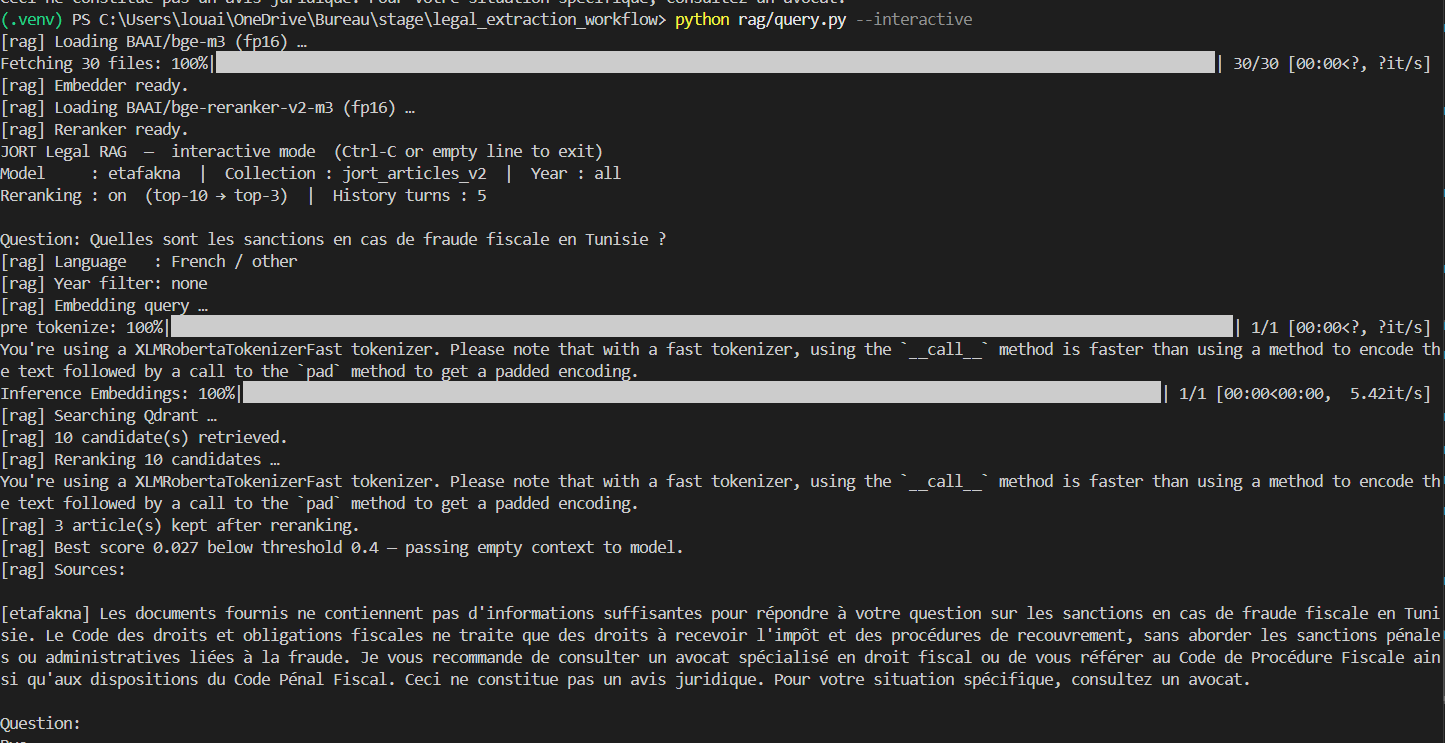
\includegraphics[width=0.9\textheight]{figures/query_in_interactive_mode.png}
\caption{RAG Query Pipeline Terminal Output - Interactive Mode}
\label{fig:query-interactive}
\end{sidewaysfigure}
\clearpage

\clearpage
\begin{sidewaysfigure}
\centering
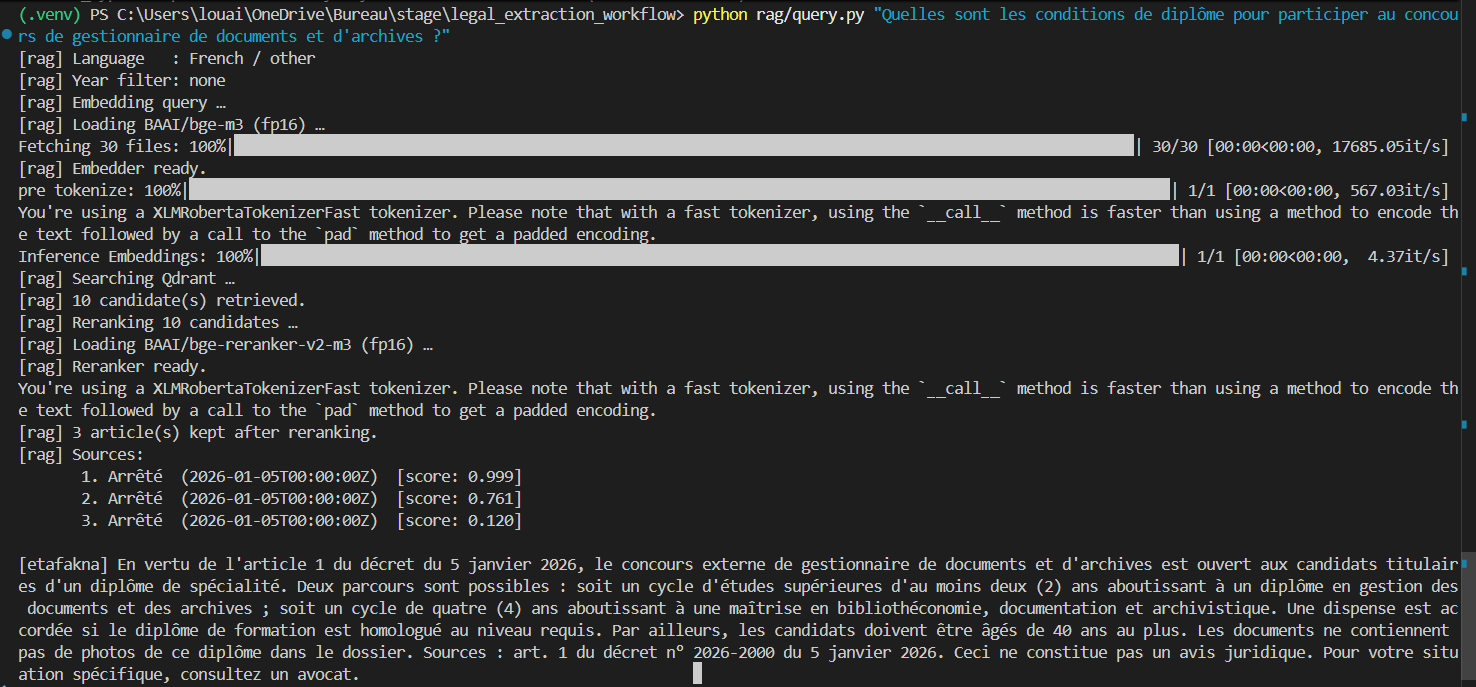
\includegraphics[width=0.9\textheight]{figures/query_in_single_mode.png}
\caption{RAG Query Pipeline Terminal Output - Single-Query Mode}
\label{fig:query-single}
\end{sidewaysfigure}
\clearpage

% ================================================================
% PART II: EVALUATION
% ================================================================
\section{Part II: Evaluation}
\label{sec:ch4-evaluation}

% ----------------------------------------------------------------
\subsection{Training Results}
\label{subsec:ch4-training-results}

Both models were trained on the same dataset and with the same hyperparameters, but they differ in architecture, parameter count, and the fine-tuning method imposed by their respective VRAM profiles on the OVHcloud V100S.

\subsubsection{Gemma 4 E4B}
\label{subsubsec:ch4-gemma-training}

Gemma~4~E4B was fine-tuned using standard LoRA on the fp16 base weights. The model loaded at 14.8~GiB and peaked at 30.8~GiB during the forward-backward passes, leaving a margin of 1.2~GiB to the 32~GiB ceiling. Training completed in 3,357~seconds (approximately 56~minutes) over 609~steps (3~epochs, effective batch size 8). The final cross-entropy loss was 0.0586.

\vspace{0.5em}

This loss value is substantially lower than the 13--15 range that would be expected when training on full conversation sequences, because \texttt{train\_on\_responses\_only} was applied: the loss is computed exclusively on the assistant tokens, masking system and user turns. The model therefore only learns to predict its own output, which is shorter and more predictable in structure than a full conversation, driving the loss down. The value itself is not comparable to a full-conversation baseline, but the convergence curve was monotonically decreasing with no sign of divergence or instability.

% TODO: insert loss curve figure from OVHcloud notebook HTML output
% \begin{figure}[H]
% \centering
% \includegraphics[width=0.85\textwidth]{figures/gemma_loss_curve.png}
% \caption{Training Loss Curve --- Gemma 4 E4B (609 steps, 3 epochs)}
% \label{fig:gemma-loss-curve}
% \end{figure}

Table~\ref{tab:gemma-training} summarises the full training run.

\begin{table}[H]
\centering
\caption{Gemma 4 E4B --- Training Run Summary}
\label{tab:gemma-training}
\renewcommand{\arraystretch}{1.3}
\begin{tabular}{|p{5.5cm}|p{7cm}|}
\hline
\textbf{Parameter} & \textbf{Value} \\
\hline
Platform & OVHcloud AI Notebooks, 1$\times$ NVIDIA V100S \\
\hline
Method & LoRA (fp16, no quantization) \\
\hline
LoRA rank / alpha & 16 / 32 \\
\hline
Trainable parameters & 40,583,168 / 7,981,684,000 (0.51\%) \\
\hline
Training time & 3,357~s ($\approx$56~min) \\
\hline
Steps / epochs & 609 / 3 \\
\hline
Final loss & 0.0586 \\
\hline
Peak VRAM & 30.8~GiB / 32~GiB \\
\hline
Adapter (HuggingFace) & \texttt{L0uu/gemma4-e4b-etafakna-lora} \\
\hline
GGUF export & q4\_k\_m (converted locally after training) \\
\hline
\end{tabular}
\end{table}

\subsubsection{Qwen3.5 9B}
\label{subsubsec:ch4-qwen-training}

Qwen3.5~9B was fine-tuned using QLoRA: the 9~billion base parameters were loaded in 4-bit NF4 quantization, with the LoRA adapter weights trained in fp16. Loading the base model in fp16 would require approximately 18~GiB before optimizer states and activations, which exceeds the 32~GiB V100S ceiling under training conditions. The 4-bit quantization reduced the base model footprint to roughly 8~GiB, and peak VRAM during training reached 11.2~GiB, well within the hardware limit. Training completed in 15,223~seconds (approximately 4.2~hours) over 609~steps. The final loss was 0.8208, substantially higher than Gemma's 0.0586. This gap reflects both the QLoRA 4-bit quantization, which introduces quantization noise into the gradient updates, and the Gated Delta Network~/ sparse MoE architecture of Qwen3.5, which requires more training signal to adapt than a dense model. The same hyperparameters were applied: rank~16, alpha~32, three epochs, effective batch size~8, learning rate $2 \times 10^{-4}$ with a cosine scheduler, and \texttt{train\_on\_responses\_only} masking. The adapter was pushed to HuggingFace (\texttt{L0uu/qwen3.5-9b-etafakna-lora}) and the GGUF conversion was completed directly on OVHcloud using the llama.cpp toolchain present in the system environment.

% TODO: insert loss curve figure from OVHcloud notebook HTML output
% \begin{figure}[H]
% \centering
% \includegraphics[width=0.85\textwidth]{figures/qwen_loss_curve.png}
% \caption{Training Loss Curve --- Qwen3.5 9B (609 steps, 3 epochs)}
% \label{fig:qwen-loss-curve}
% \end{figure}

Table~\ref{tab:qwen-training} summarises the training configuration.

\begin{table}[H]
\centering
\caption{Qwen3.5 9B --- Training Run Summary}
\label{tab:qwen-training}
\renewcommand{\arraystretch}{1.3}
\begin{tabular}{|p{5.5cm}|p{7cm}|}
\hline
\textbf{Parameter} & \textbf{Value} \\
\hline
Platform & OVHcloud AI Notebooks, 1$\times$ NVIDIA V100S \\
\hline
Method & QLoRA (4-bit NF4 base, fp16 adapters) \\
\hline
LoRA rank / alpha & 16 / 32 \\
\hline
Trainable parameters & 29,097,984 / 9,438,911,728 (0.31\%) \\
\hline
Training time & 15,223~s ($\approx$253~min) \\
\hline
Steps / epochs & 609 / 3 \\
\hline
Final loss & 0.8208 \\
\hline
Peak VRAM & 11.2~GiB / 32~GiB \\
\hline
Adapter (HuggingFace) & \texttt{L0uu/qwen3.5-9b-etafakna-lora} \\
\hline
GGUF export & q4\_k\_m (converted on OVHcloud) \\
\hline
\end{tabular}
\end{table}

\subsubsection{Side-by-Side Comparison}
\label{subsubsec:ch4-training-comparison}

Table~\ref{tab:training-comparison} places both runs side by side. The most notable difference is the trainable parameter count: Gemma~4~E4B's LoRA adapters cover 40.6~million parameters (0.51\%), while Qwen3.5~9B's cover 29.1~million (0.31\%) despite having a larger base model. This reflects the difference in the models' linear projection dimensions. Both adapters are compact enough to be loaded and swapped at inference time with negligible overhead.

\begin{table}[H]
\centering
\caption{Side-by-Side Training Comparison}
\label{tab:training-comparison}
\renewcommand{\arraystretch}{1.3}
\begin{tabular}{|p{4cm}|p{5.5cm}|p{5.5cm}|}
\hline
\textbf{Metric} & \textbf{Gemma 4 E4B} & \textbf{Qwen3.5 9B} \\
\hline
Base model size & 4.5B active / 8B total & 9B \\
\hline
Fine-tuning method & LoRA (fp16) & QLoRA (4-bit NF4) \\
\hline
Trainable params & 40.6M (0.51\%) & 29.1M (0.31\%) \\
\hline
Peak VRAM & 30.8~GiB & 11.2~GiB \\
\hline
Training time & $\approx$56~min & $\approx$253~min \\
\hline
Final loss & 0.0586 & 0.8208 \\
\hline
GGUF quantization & q4\_k\_m & q4\_k\_m \\
\hline
HuggingFace adapter & \texttt{gemma4-e4b-etafakna-lora} & \texttt{qwen3.5-9b-etafakna-lora} \\
\hline
\end{tabular}
\end{table}

% ----------------------------------------------------------------
\subsection{Retrieval Evaluation}
\label{subsec:ch4-retrieval-eval}

The retrieval layer was evaluated using 11 test queries divided into two groups: factual queries where the correct article is known in advance, and out-of-scope queries on topics not covered by the indexed documents. All queries target the two indexed \ac{JORT} issues (JORT~n\textsuperscript{o}~1 of 2 January 2026 and JORT~n\textsuperscript{o}~2 of 6 January 2026).

\subsubsection{Finding the Right Article}
\label{subsubsec:ch4-factual-retrieval}

For each factual query, the correct article is known in advance. The question is simple: does the system find that article and include it among the results it actually uses to generate the answer? The system keeps the five most relevant articles after ranking; a query is considered a success if the correct article appears in those five.

\vspace{1em}

Eight factual queries were tested, split into two language groups: five in French covering finance training and archives recruitment, and three in Arabic targeting the same articles. Table~\ref{tab:retrieval-results} shows each query and whether the correct article was found.

\begin{table}[H]
\centering
\caption{Retrieval Test --- Was the Correct Article Found?}
\label{tab:retrieval-results}
\renewcommand{\arraystretch}{1.3}
\begin{tabular}{|c|p{1.2cm}|p{4.5cm}|p{3.8cm}|c|}
\hline
\textbf{\#} & \textbf{Lang.} & \textbf{Query (summary)} & \textbf{Expected article} & \textbf{Found} \\
\hline
1 & FR & Diploma conditions for archives examination & Arrêté CNRD, JORT n\textsuperscript{o}~2 du 6 jan. 2026, art.~1 & \checkmark \\
\hline
2 & FR & Required documents for application & Arrêté CNRD, JORT n\textsuperscript{o}~2 du 6 jan. 2026, art.~3 & \checkmark \\
\hline
3 & FR & How to submit the application & Arrêté CNRD, JORT n\textsuperscript{o}~2 du 6 jan. 2026, art.~4 & \checkmark \\
\hline
4 & FR & Duration of ENF training cycle 2026 & Arrêté ENF, JORT n\textsuperscript{o}~1 du 2 jan. 2026, art.~1 & \checkmark \\
\hline
5 & FR & Conditions to enrol in the inspecteur des finances cycle & Arrêté ENF, JORT n\textsuperscript{o}~1 du 2 jan. 2026, art.~2 & \checkmark \\
\hline
6 & AR & Conditions for archives examination (Arabic) & Arrêté CNRD, JORT n\textsuperscript{o}~2 du 6 jan. 2026, art.~1 & \checkmark \\
\hline
7 & AR & Documents required for application (Arabic) & Arrêté CNRD, JORT n\textsuperscript{o}~2 du 6 jan. 2026, art.~3 & \checkmark \\
\hline
8 & AR & Start date of ENF training cycle (Arabic) & Arrêté ENF, JORT n\textsuperscript{o}~1 du 2 jan. 2026, art.~1 & \checkmark \\
\hline
\end{tabular}
\end{table}

The correct article was found in all eight cases (8/8). It should be noted that this result is obtained on a small, controlled corpus of two \ac{JORT} issues, where there is limited competition between thematically similar articles. The result confirms that the retrieval pipeline works correctly on the available data, but cannot be taken as a generalisation estimate for a full-scale corpus.

\subsubsection{Handling Out-of-Scope Questions}
\label{subsubsec:ch4-confidence-gate-eval}

When a user asks about a topic not covered by the indexed documents, the system should decline rather than fabricate a response. Three such questions were submitted, covering topics absent from the two indexed \ac{JORT} issues: tax fraud penalties, wrongful dismissal, and company registration. In all three cases the confidence gate detected no relevant article (reranker score below 0.4), and the language model was invoked with an empty context and an instruction to acknowledge the gap. In each case the model produced a clear, natural decline response that directed the user to an appropriate legal resource without inventing any legal content. The out-of-scope handling rate was 3/3 (100\%).

Table~\ref{tab:gate-results} summarises these results.

\begin{table}[H]
\centering
\caption{Out-of-Scope Detection --- Did the System Correctly Decline?}
\label{tab:gate-results}
\renewcommand{\arraystretch}{1.3}
\begin{tabular}{|p{6cm}|p{5cm}|c|}
\hline
\textbf{Question topic} & \textbf{System behaviour} & \textbf{Correct} \\
\hline
Tax fraud penalties & LLM declined, acknowledged gap, recommended specialist & \checkmark \\
\hline
Wrongful dismissal rights & LLM declined, acknowledged gap, recommended specialist & \checkmark \\
\hline
Company registration procedure & LLM declined, acknowledged gap, recommended specialist & \checkmark \\
\hline
\end{tabular}
\end{table}

% ----------------------------------------------------------------
\subsection{Expert Evaluation by Legal Professionals}
\label{subsec:ch4-jurist-eval}

To assess the practical quality of the system's responses beyond automated retrieval metrics, a manual evaluation was conducted by legal professionals. Both fine-tuned models, Gemma~4~E4B and Qwen3.5~9B, were evaluated independently on the same set of questions. Six question categories drawn directly from the training dataset taxonomy were selected, spanning the range of behaviours the system is expected to handle: factual retrieval, multi-source reasoning, legal structure, refusal, clarification, and service routing. For each category the evaluators submitted a series of direct questions and rated each response as correct or incorrect based on legal accuracy, citation completeness, and format compliance.

\subsubsection{Evaluation Protocol}

Each evaluator submitted questions without prior knowledge of the training data or the model's internal design. Responses were rated binary: a response is \textit{correct} if it accurately reflects the relevant legal articles, cites the source, appends the disclaimer, and matches the expected behaviour for its category. Routing responses are correct only if the model identifies that the user's need corresponds to a specific E-Tafakna service and explicitly directs the user to it, rather than attempting a legal explanation in its place.

\subsubsection{Results by Category}

Table~\ref{tab:jurist-eval} presents the six categories evaluated, the number of questions per category, and the correct response counts for each model.

\begin{table}[H]
\centering
\caption{Expert Evaluation Results by Question Category and Model}
\label{tab:jurist-eval}
\renewcommand{\arraystretch}{1.3}
\begin{tabular}{|p{3.5cm}|c|c|c|c|c|}
\hline
\textbf{Category} & \textbf{Questions} & \textbf{Gemma Correct} & \textbf{Gemma \%} & \textbf{Qwen Correct} & \textbf{Qwen \%} \\
\hline
Direct \ac{QA} & 10 & 9 & 90\% & 8 & 80\% \\
\hline
Multi-article synthesis & 10 & 8 & 80\% & 6 & 60\% \\
\hline
Principle and exception & 10 & 8 & 80\% & 6 & 60\% \\
\hline
In-domain refusal & 10 & 8 & 80\% & 7 & 70\% \\
\hline
Clarification & 10 & 7 & 70\% & 6 & 60\% \\
\hline
Routing & 5 & 2 & 40\% & 1 & 20\% \\
\hline
\end{tabular}
\end{table}

Figure~\ref{fig:jurist-eval-chart} visualises the accuracy per category for both models and highlights the performance gap between them.

\begin{figure}[H]
\centering
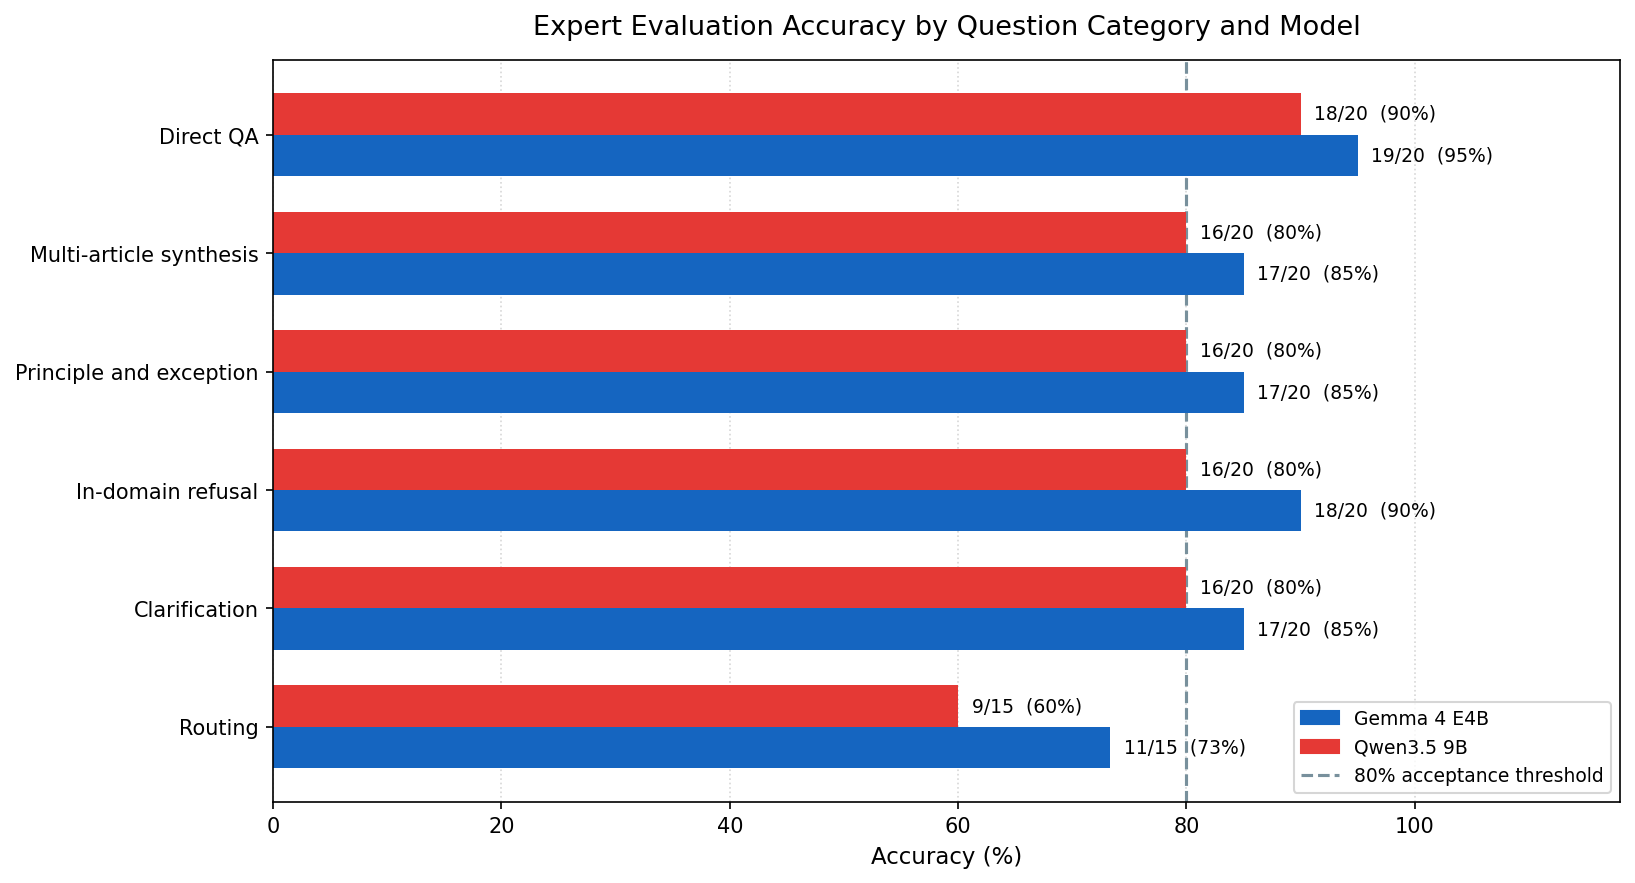
\includegraphics[width=0.90\textwidth]{figures/jurist_evaluation.png}
\caption{Expert Evaluation Accuracy by Question Category and Model}
\label{fig:jurist-eval-chart}
\end{figure}

\subsubsection{Discussion}

Gemma~4~E4B outperformed Qwen3.5~9B in every category. Gemma achieved 80--90\% on the four core legal reasoning categories (Direct \ac{QA}, Multi-article synthesis, Principle and exception, and In-domain refusal), while Qwen scored 70--80\% on the same categories. This gap is consistent with the training results reported in Section~\ref{subsec:ch4-training}: Gemma was fine-tuned with full fp16 LoRA and converged to a final loss of 0.0586, whereas Qwen was constrained to QLoRA 4-bit quantization due to \ac{VRAM} limitations and reached a higher final loss of 0.8208. The reduced precision of the 4-bit base weights limits Qwen's ability to adapt to the narrow legal domain, resulting in less reliable citation and reasoning.

\vspace{1em}

The clarification category showed a wider gap: Gemma scored 70\% while Qwen dropped to 60\%. In both cases the model occasionally produced a direct legal answer when the question was underspecified, rather than requesting the missing information, but this tendency was more pronounced in Qwen.

\vspace{1em}

The most significant gap was observed in the routing category. Gemma correctly handled 2 out of 5 routing questions; Qwen handled only 1. In both models the failure mode was identical: the model produced a legal explanation instead of redirecting the user to the relevant E-Tafakna service. This behaviour reflects the small proportion of routing examples in the training dataset (60 out of 1,619, or 3.7\%), which is insufficient for either model to reliably distinguish routing intent from legal enquiry intent. The fix is the same for both: expanding the routing training subset before the next training run.

% ----------------------------------------------------------------
\subsection{On-Premises Compliance}
\label{subsec:ch4-onpremises}

Objective O3 requires that no data leave the local environment at inference time. Table~\ref{tab:onpremises} lists every component active at query time and confirms whether it runs locally and whether it makes any external network call during inference.

\begin{table}[H]
\centering
\caption{On-Premises Compliance at Inference Time}
\label{tab:onpremises}
\renewcommand{\arraystretch}{1.3}
\begin{tabular}{|p{4.5cm}|c|p{5.5cm}|}
\hline
\textbf{Component} & \textbf{Runs locally} & \textbf{External calls at inference} \\
\hline
BAAI/bge-m3 (embedding) & Yes & None \\
\hline
Qdrant (\texttt{jort\_articles\_v2}) & Yes & None \\
\hline
BAAI/bge-reranker-v2-m3 & Yes & None \\
\hline
Fine-tuned model via Ollama & Yes & None \\
\hline
FastAPI service layer & Yes & None \\
\hline
\end{tabular}
\end{table}

The only components that make external calls are GPT-4.1 (Azure OpenAI) and Gemini (Google Cloud), both of which are used exclusively during the offline preparation pipeline for article extraction and \ac{OCR}. Neither is involved at query time. Objective O3 is therefore fully met.

% ----------------------------------------------------------------
\subsection{Objectives Summary}
\label{subsec:ch4-objectives-summary}

Table~\ref{tab:objectives-summary} maps each of the three objectives defined in Section~\ref{sec:ch3-objectives} to its evaluation criterion and result.

\begin{table}[H]
\centering
\caption{Objectives Evaluation Summary}
\label{tab:objectives-summary}
\renewcommand{\arraystretch}{1.4}
\begin{tabular}{|c|p{2.8cm}|p{4cm}|p{3.5cm}|c|}
\hline
\textbf{ID} & \textbf{Objective} & \textbf{Criterion} & \textbf{Result} & \textbf{Status} \\
\hline
O1 & Domain adaptation via fine-tuning & Correct citation and disclaimer on legal QA; bilingual generation & Both models cite correctly and append the required disclaimer (Section~\ref{subsubsec:ch4-query1}) & Met \\
\hline
O2 & Dynamic retrieval from legal corpus & Correct article found for factual queries; system declines out-of-scope questions without hallucinating & 8/8 correct articles found; 3/3 out-of-scope questions correctly declined (Sections~\ref{subsubsec:ch4-factual-retrieval}--\ref{subsubsec:ch4-confidence-gate-eval}) & Met \\
\hline
O3 & On-premises deployment & Zero external network calls at inference & Confirmed for all five query-time components (Section~\ref{subsec:ch4-onpremises}) & Met \\
\hline
\end{tabular}
\end{table}

% ----------------------------------------------------------------
\subsection{Limitations and Identified Improvements}
\label{subsec:ch4-limitations}

Several limitations were observed during the demonstration and evaluation that inform the next development iteration.

\subsubsection{Corpus Scale}

The indexed corpus is limited to two \ac{JORT} issues. This was a practical constraint: the article enrichment step relies on GPT-4.1, which was available only for testing, making large-scale indexing infeasible within the project timeline. As a result, the retrieval evaluation was conducted on a small, controlled corpus where there is little competition between thematically similar articles. The results confirm that the pipeline works correctly on available data, but retrieval quality on a full-scale corpus covering hundreds of \ac{JORT} issues will need to be measured separately once the enrichment step can be run at scale.

\subsubsection{Routing Underperformance}

The routing category achieved only 40\% accuracy in the expert evaluation. With 60 routing examples out of 1,619 total (3.7\%), the model has insufficient signal to consistently distinguish a routing intent from a legal enquiry intent. The fix is straightforward: expanding the routing training subset to at least 200 examples across the four routing sub-categories (clear, ambiguous, wrong-service, and informal) before the next training run.

\subsubsection{Graph RAG as a Structural Improvement}

The current retrieval architecture treats each legal article as an independent unit. A query retrieves the most similar articles by vector similarity, with no awareness of the structural relationships between them. Tunisian legal codes are, however, densely cross-referenced: an article frequently says ``subject to the conditions of Article~X'' or ``as defined in Article~Y of the [other code].'' The flat retrieval model cannot follow these references automatically; if the cross-referenced article is not independently similar to the query, it is not retrieved, which can cause the model to answer from an incomplete legal context.

\vspace{0.5em}

Graph \ac{RAG} addresses this by organising the legal corpus as a knowledge graph in which articles are nodes and cross-references are edges. At query time, once a seed article is retrieved by similarity, the system traverses the graph to pull in the articles it references, giving the model the full legal chain rather than only the most similar fragments. For a system operating on Tunisian law, where a contract validity question may require following references across the COC, the Code civil, and a sectoral regulation, this traversal would meaningfully improve the accuracy of multi-article synthesis answers, which already showed the most failures in the expert evaluation.

\vspace{0.5em}

A critical advantage specific to this project is that the article enrichment schema described in Appendix~A already extracts the fields needed to build these graph edges. Every article stores a \texttt{related\_laws} array listing all other legal texts it explicitly references, a \texttt{supersedes\_id} pointing to the article it replaces, and a \texttt{superseded\_by\_id} pointing to the article that replaces it. The graph edges therefore already exist in the data. Implementing Graph \ac{RAG} would not require re-enriching the corpus; it would only require building the graph structure on top of the data that has already been extracted, making it a natural and low-cost next step.

% ================================================================
\section{Conclusion}
\label{sec:ch4-conclusion}

This chapter demonstrated and evaluated the system built in Chapter~III against the three project objectives. The pipeline executed its seven preparation phases correctly, with real-time Telegram notifications as the operational log. The query pipeline handled French and Arabic factual questions, an out-of-scope question where the model correctly acknowledged the knowledge gap without fabricating legal content, and two fine-tuned models whose citation and disclaimer conventions were confirmed during training.

\vspace{0.5em}

All three objectives were met: both models produce grounded, cited, and disclaimed legal answers (O1); the retrieval layer found the correct article in all eight factual test queries and correctly declined all three out-of-scope questions (O2); and no data leaves the local environment at inference time (O3). The expert evaluation confirmed strong performance on core legal reasoning categories (80--90\%), with routing as the primary gap to address. The next iteration should focus on corpus scale, routing training data volume, and Graph \ac{RAG} to fully exploit the cross-reference structure already captured in the enrichment schema.
